%\section{Selection Cuts for eleTau Channel}
\section{\texorpdfstring{Event selection for the \leptonTau channel}{Event selection for the lepton-tau channel}}
\label{sect:eleTauCuts}
Events for the \leptonTau final states (e\Tau and $\mu\Tau$)
were collected with triggers that require 
a loosely isolated \Tau with \PT $>$ 20 \GeV and $|\eta|$ $<$ 2.3 as well as
an isolated electron or muon with $|\eta| < 2.1$.  The minimum
\PT requirement for the electron (muon) was increased during the data taking from 20 to 22 \GeV (17 to 18 \GeV)
due to the increase in instantaneous luminosity.

In the offline analysis the electron, muon, and \Tau objects were required to have \PT $>$ 25, 20, and 25 \GeV, respectively, 
while tightening the corresponding identification and isolation requirements.
In events with more than one opposite-sign \leptonTau pair, we only consider
 the pair that maximizes the scalar sum of \Tau and electron or muon 
transverse momenta.  Events with an additional loosely isolated lepton
with \PT $>$ 10 \GeV are rejected to suppress backgrounds from $Z$ boson
decays.  

Just as for the \Tau\Tau channel we apply preselection requirements to suppress
QCD and \ttbar events, $Z \to \tau \tau$ decays, and low mass resonances.
These requirements are: \mttwo $>$ 40 \GeV, \MPT $>$ 30 GeV, \leptonTau 
invariant mass between 15 and 45 \GeV or $>$ 75 \GeV, $\Delta \Phi > 1$, and we veto events with b-tagged jets.
The final signal region requirements are \mttwo $>$ 90 \GeV and 
\tauMT $>$ 200 \GeV. %where \tauMT is the \Tau transverse mass 
The latter requirement provides discrimination against the \wjets background.  Unlike the \tauTau channel,
events with \mttwo $<$ 90 \GeV are not used because of the higher 
level of background.


Figure \ref{fig:mt2leptontau} % and \ref{fig:taumtleptontau} 
shows the \mttwo distribution after the preselection.
%and the \tauMT distribution after the preselection and the \mttwo requirements, respectively.
The data are in good agreement with the SM expectations. A SUSY signal corresponding to a high mass difference 
 $(m_{\chione}=380\GeV,~m_{\PSGczDo}=1\GeV)$ is used to show the expected signal distribution.

\begin{figure}[!Hhtb]
\centering
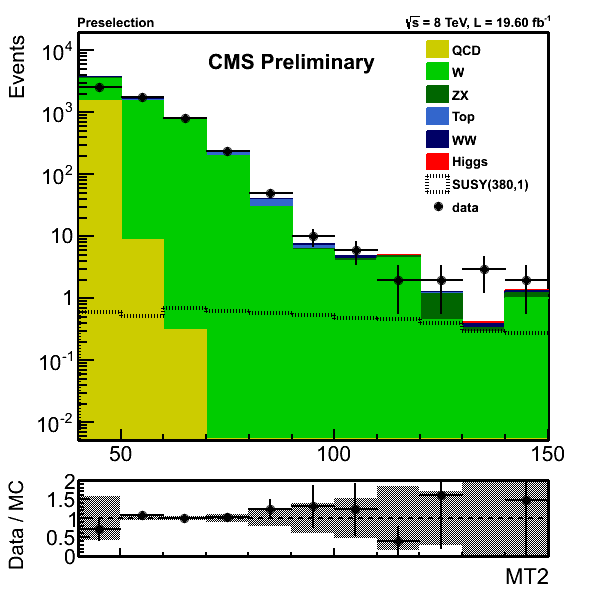
\includegraphics[angle=0,scale=0.35]{SelectionEleTau/MT2.png}
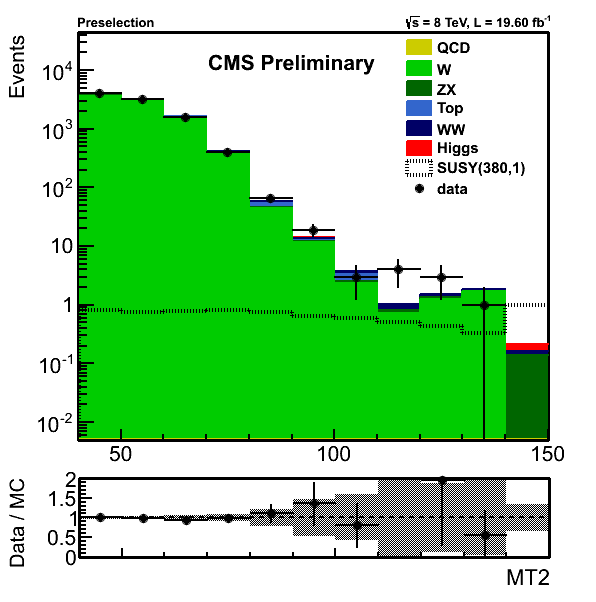
\includegraphics[angle=0,scale=0.35]{SelectionMuTau/MT2_Ratio_Preselection_unBlinded.png}
\caption{\mttwo  distributions for events in the preselection sample, compared to Monte Carlo events in (left) \eTau and (right) \muTau channels. The signal point shown here is $(m_{\chione}=380\GeV,~m_{\PSGczDo}=1\GeV)$.}
\label{fig:mt2leptontau}
\end{figure}

